\newpage
\section{Evaluation}
\label{sec:eval}
%
\begin{figure}[b]
\centering
\begin{center}
\begin{scriptsize}
\begin{tabular}{|l |  l | l|} 
\hline
 \multicolumn{1}{|c}  {\bf Benchmark} & \multicolumn{1}{c} {\bf
 Consistency} & \multicolumn{1}{c|}  {\bf
 Description}\\ [0.5ex] 
\hline
Counter  & MR & {Monotonicly increasing counter, e.g.
YouTubes' watch 
count}\\ \hline
DynamoDB  & RMW & {Integer register allowing various conditional puts and gets} \\ \hline
Online Store & RMW &  {Online store with shopping carts
and modifiable item prices} \\ \hline
Bankaccount  & 2VIS $\wedge$ RMW & {Offering deposit, withdraw and get balance operations}\\ \hline
Shopping List   &  MW $\wedge$ RMW & {A shopping list with
concurrent adds and deletes functionality}\\ \hline 
Microblog  &  MW, RMW & {A Twitter-like application modeled after
Twissandra}\\\hline
Rubis  & RMW, RMW$\wedge$2VIS & {eBay-like
application with browsing, supporting user wallet} \\
\hline
\end{tabular}
\end{scriptsize}
\end{center}
\caption{Fine-grained consistency requirement in benchmark programs}
\label{fig:dist_table}
\end{figure}

%intro: benchmark programs
In this section we present an evaluation study of our implementation,
including a report on
benchmark applications that utilize fine-grained weak consistency
requirements, expressable
in our specification language.
Fig.~\ref{fig:dist_table} presents seven of such programs, including
individual data types as well as larger programs consisted of multiple
data types. 

%multiple consistency levels for each program
Each program offers various operations, each of which is assigned a
potentially different consistency requirement,
representing the need for a multi-consistnet environement for
efficient execution of the programs. Surprisingly, we found no program
requiring causal consistency; all known consistency anomalies that operations
may be involved in, are expressable with simple contracts made of
dependency relations of length 1 or 2,
which differs from what was knwon in the context before, where all such
operations were considered to require CC.

%conjunction of consistency requirements for even a single operation
Additionally, in many cases we found operations that are involved in
multiple anomalies, requiring simultaneous enforcement of different
consistency guarantees, which shows the unfeasability of hand-writing
such guarantees, considering the vast set  of known consistency
anomalies. 
%
%example
For example, consider the bank account application, which offers
\dRV{}, \wdRV{} and \gbRV{} operations, where a \wdRV{} is a
strongly consistent operation that succeeds only if there are sufficient
funds in the account. There are two annomalies associate with
\gbRV{} in this program:
\begin{enumerate*}[label=(\roman*)]
\item when a users performs a \dRV{}, which is however, not refleceted
in the subsequent \gbRV{}
\item when a \gbRV{} witnesses a \wdRV{} effect, without witnessing all
the \dRV{} effects that were visible to it,
which may result in \gbRV{} returning a
negative balance.
\end{enumerate*}
As it is presented in Fig.~\ref{fig:dist_table}, in order to preempt
these anomalies, \gbRV{} requires
both \rmwCTRT{} and \visCTRT{} guarantees.
\begin{figure}[t]
        \centering
	\begin{subfigure}[t]{0.25\textwidth}
	\centering
	\hspace{-13mm}
	
\includegraphics[scale=0.22]{Figures/latency.pdf}
	\subcaption*{ \hspace{-10mm} (a) Latency}
	\end{subfigure}
	\begin{subfigure}[t]{0.36\textwidth}
	\centering
	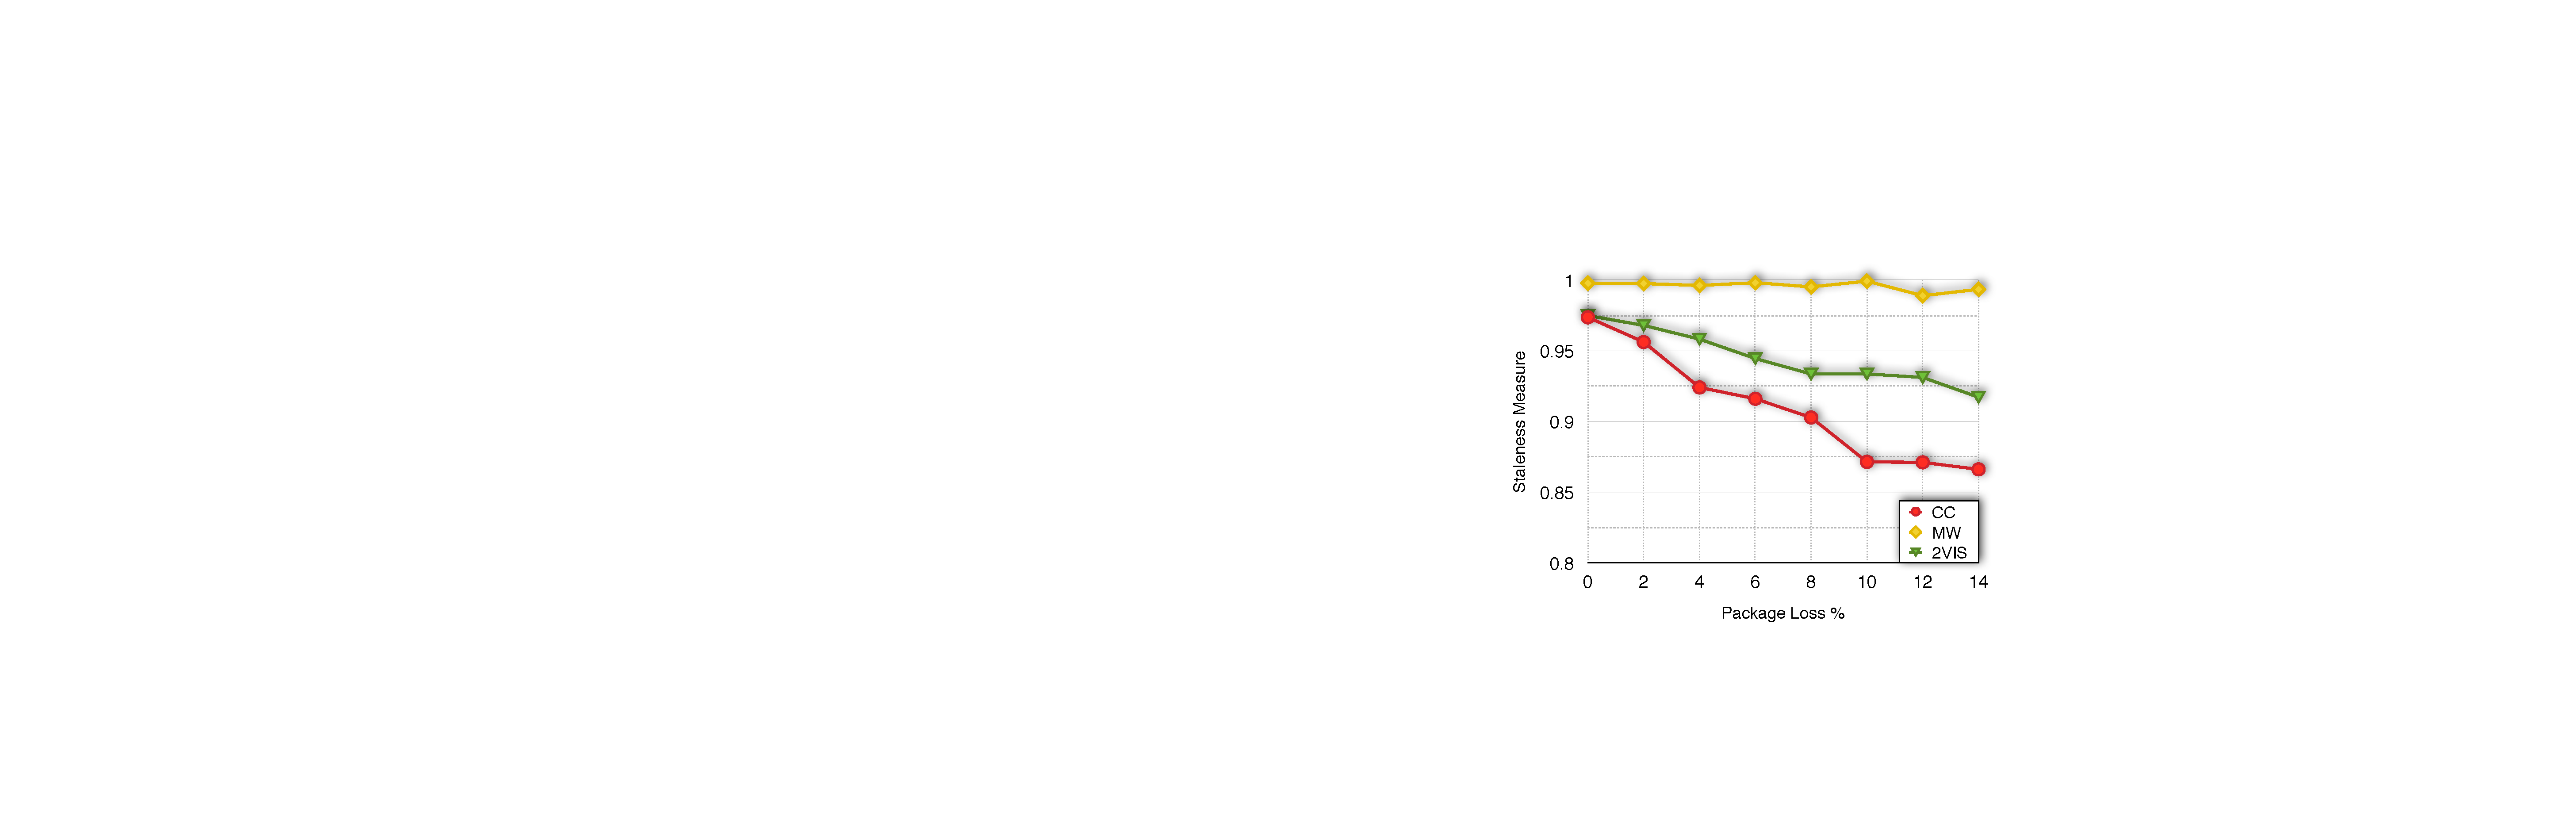
\includegraphics[scale=0.22]{Figures/staleness.pdf}
	\subcaption*{ \hspace{-1mm} (b) Staleness}
	\label{subfig:comment_example}
	\end{subfigure} 
	\begin{subfigure}[t]{0.28\textwidth}
	\centering
	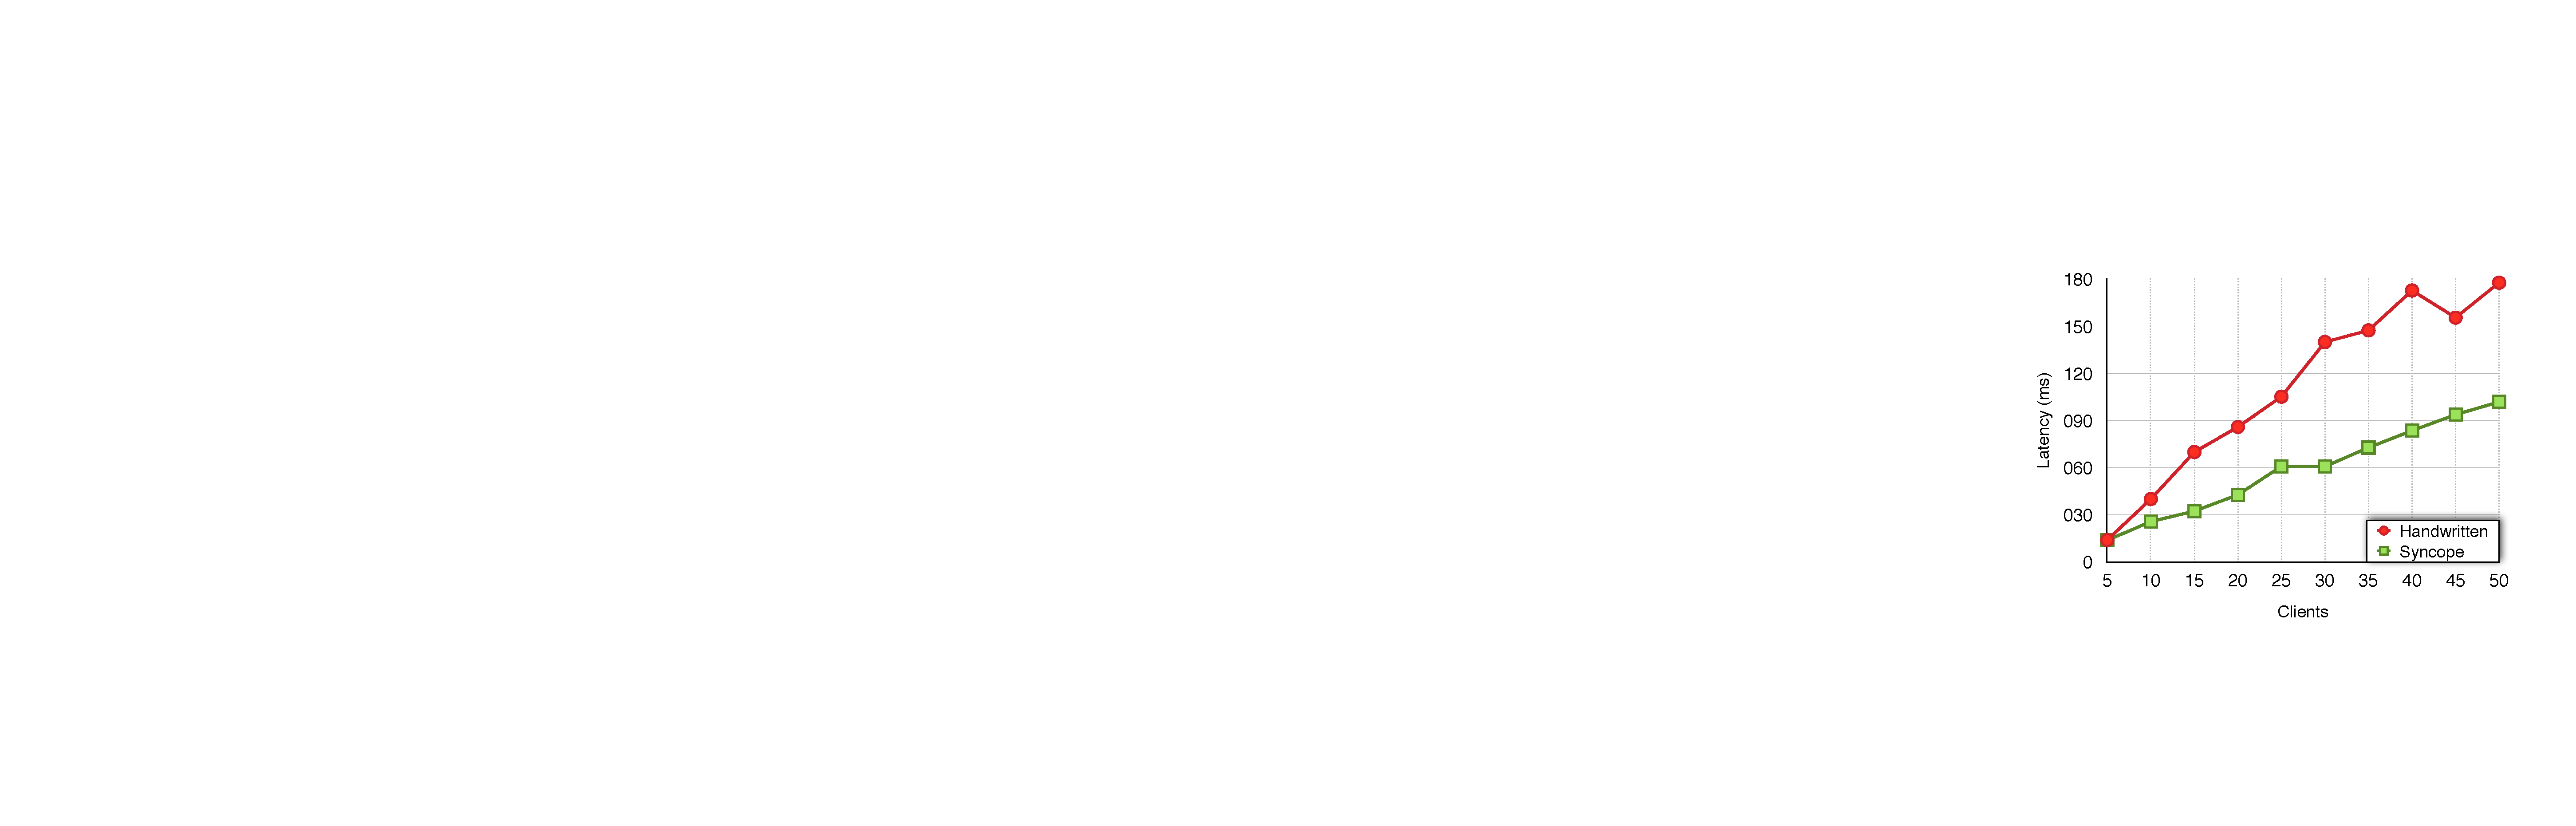
\includegraphics[scale=0.22]{Figures/comparison.pdf}
	\subcaption*{ \hspace{8mm} (c) Manual RMW}
	\label{subfig:comment_example}
	\end{subfigure} 
\\ \hrulefill
\caption{A distributed application for comment section
management}
\label{fig:eval}
\end{figure}



% performance evaluation
To evaluate its performance, we deploy \tool on a cloud cluster,
consisting of three fully replicated Cassandra replicas, running on
seperate machines within the same
datacenter. 
Each machine is instantiated with a
\tool shim layer, that responds to clients,  
 which are instantiated on a virtual machine 
co-located with one of the replicas on a machine.
We deploy the cluster on three \texttt{m4.4xlarge} Amazon EC2 instances
in US-West (Oregon) region, with inter-machine communication time of 5ms.

% The problem with Cassandra
Since Cassandra is developed over TCP connections for replica communications, 
we found all messages being  delivered with no loss and in order, making
it much more consistent  than  EC, and masking out the
differences between our fine-grained consistency guarantees.
Consequently, to simulate a
realistic EC environment, we inject random message losses at the shim
layers, where a message delivery is delayed for 1
second in case it is lost.

%The latency and staleness gain using fine-grained consistency
Fig.~\ref{fig:eval}(a) and \ref{fig:eval}(b) represent
our experimental results, with a workload generated 
by 50 concurrent clients repeatedly running sessions, each composed of three
operations, where operations uniformly choose from 5 objects and are
performed under the specified consistency level. 
We increased the
percentage of delayed messages from 0 to 14, and each experiment ran for
100 repeaded sessions per client, where the staleness measure is the
the ratio of the number of visible effects, 
to all available effects, averaged on all operations at all
replicas.

The first set of experiments, measures the client perceived latency for
three different \LB{} contracts all implemented in \tool. As expected,
causal consistency, the strongest consistency level our tool can
enforce,  experiences the larges increase in latency. The results show
$17\%$ and $67\%$ increase in latency between (RMW-MR) and (MR-CC) at only
$4$ percent message loss. These numbers go up to respectively $18\%$ and
$87\%$ at $10$ percent message loss.
















































